%% Author    :  CHARLES Clarence Dimitri



\documentclass[a4paper,14pt]{article}
\usepackage[french]{babel}
\usepackage[utf8]{inputenc}
\usepackage{times}
\usepackage{url}
\usepackage{amsmath}
\usepackage{amssymb}
\usepackage{underscore}
\usepackage[T1]{fontenc}            %% Csure des mots accentus (Hyphenation)
\usepackage{ulem}               %% Souligner deux fois
\usepackage{listings}           %% Code  
\usepackage{graphicx}
%\usepackage{algorithmic}
%\usepackage{algorithm}
\usepackage{color}
\usepackage{pifont}
\definecolor{colKeys}{rgb}{0,0,1}
\definecolor{colIdentifier}{rgb}{0,0,0}
\definecolor{colComments}{rgb}{0,0.5,1}
\definecolor{colString}{rgb}{0.6,0.1,0.1}



\lstset{
basicstyle=\ttfamily\small, %
identifierstyle=\color{colIdentifier}, %
keywordstyle=\color{colKeys}, %
stringstyle=\color{colString}, %
commentstyle=\color{colComments},
numbers=left,                   % where to put the line-numbers
numberstyle=\footnotesize,      % the size of the fonts that are used for the line-numbers
stepnumber=1,                   % the step between two line-numbers. If it's 1 each line will be numbered
numbersep=5pt,                  % how far the line-numbers are from the code
showspaces=false,               % show spaces adding particular underscores
showstringspaces=false,         % underline spaces within strings
showtabs=false,                 % show tabs within strings adding particular underscores
frame=single,	                % adds a frame around the code
tabsize=2,	                % sets default tabsize to 2 spaces
captionpos=b,                   % sets the caption-position to bottom
breaklines=true,                % sets automatic line breaking
breakatwhitespace=false,        % sets if automatic breaks should only happen at whitespace
title=\lstname,                 % show the filename of files included with \lstinputlisting; also try caption instead of title
escapeinside={\%*}{*)} ,         % if you want to add a comment within your code
morecomment=[s]{/*}{*/}
}
\lstset{language=java} 


%% Creation d'un format pour le titre
\makeatletter
\def\maketitle{%
  \thispagestyle{empty}\vbox to \vsize{%
    \vfill
    \vspace{1cm}
    \begin{flushleft}
      \usefont{OT1}{ptm}{m}{n}
      \huge \@title
    \end{flushleft}
    \par
    \hrule height 4pt
    \par
    \begin{flushright}
      \usefont{OT1}{phv}{m}{n}
      \Large \@author
      \par
    \end{flushright}
    \vspace{1cm}
    \vfill
    \vfill
    \bf{Le \@date}
  }%
  \cleardoublepage
}



% On definit le symbole IN
\def\N{\mbox{I\hspace{-.15em}N}} 

%%% francisation des algorithmes
%\renewcommand{\algorithmicrequire} {\textbf{\textsc{Entres:}}}
%\renewcommand{\algorithmicensure}  {\textbf{\textsc{Sorties:}}}
%\renewcommand{\algorithmicwhile}   {\textbf{tantque}}
%\renewcommand{\algorithmicdo}      {\textbf{faire}}
%\renewcommand{\algorithmicendwhile}{\textbf{fin tantque}}
%\renewcommand{\algorithmicend}     {\textbf{fin}}
%\renewcommand{\algorithmicif}      {\textbf{si}}
%\renewcommand{\algorithmicendif}   {\textbf{finsi}}
%\renewcommand{\algorithmicelse}    {\textbf{sinon}}
%\renewcommand{\algorithmicthen}    {\textbf{alors}}
%\renewcommand{\algorithmicfor}     {\textbf{pour}}
%\renewcommand{\algorithmicforall}  {\textbf{pour tout}}
%\renewcommand{\algorithmicdo}      {\textbf{faire}}
%\renewcommand{\algorithmicendfor}  {\textbf{fin pour}}
%\renewcommand{\algorithmicloop}    {\textbf{boucler}}
%\renewcommand{\algorithmicendloop} {\textbf{fin boucle}}
%\renewcommand{\algorithmicrepeat}  {\textbf{rpter}}
%\renewcommand{\algorithmicuntil}   {\textbf{jusqu'}}



% Csures
\hyphenation{meta-don-nees}


% Inclusion du dossier des figures
\graphicspath{{./figure/}}


\title{Édition de modèles en mode multi-vues dans un contexte distribué et déconnecté}
\author{CHARLES Clarence Dimitri}
\begin{document}

\maketitle
\tableofcontents
\cleardoublepage

\section{Introduction}
MDE (Model Driven Engineering) est une démarche de développement logiciel s'appuyant sur les modèles. Cette approche, très répandue dans le milieu industriel, s'utilise de plus en plus dans les projets  large échelle et dans un contexte distribué. Ces projets requièrent la collaboration de plusieurs équipes de développement réparties géographiquement éditant le même modèle. Dans un tel contexte, certains problèmes se posent. \newline
Le premier problème qui se pose concerne la réplication partielle de modèles. Jusqu'à présent, 
la totalité du modèle était répliquée sur les postes de développeurs, c'est-à-dire que chaque poste de développeur contenait la globalité du modèle sur sa machine 
même si ce dernier n'était intéressé que par un aspect du modèle. Certains projets pouvant atteindre des centaines, voir des milliers de classes, il y' donc une nécessité de mettre en place
un outil pour la réplication partielle de modèles. C'est-à-dire, que chaque développeur aura dans son espace de travail que le morceau de modèle qui l'intéresse.
Le 2ème problème est celui de la cohérence. Nous rappelons que les équipes impliquées dans un projet éditent concurremment le même modèle. Supposons qu'une équipe A travaille sur un
composant offrant une interface qui est utilisée par d'autres équipes. Si l'équipe A modifie cette interface (ajout/suppression de méthodes, changement de type de paramètres, etc), 
il est important que les autres aient une version mise  jour de cette interface. Supposons qu'une équipe B travaille sur le même composant et 
modifie aussi ladite interface en même temps que A, quels changements
seront pris en compte? Le problème devient compliqué lorsque A et B travaillent en même temps sur sur les mêmes éléments (par exemple A supprime un élément et B rajoute une référence  cet élément). Comment garder la consistance de cette interface entre A et B et les différentes équipes la partageant?
Le 3ème problème est celui du travail en mode non-connecté. Les modèles sont dits par plusieurs équipes ne travaillant pas tous en même en temps, soit pour des raisons géographiques, soit pour des contraintes horaires, etc. Un développeur peut aussi décider  tout moment de se déconnecter et travailler en local. Lorsqu'il se reconnectera, il soumettra son travail aux autres membres de son équipe. Des conflits pouvant émerger lors de cette soumission donc il faudra réfléchir sur la gestion de ces conflits en exploitant les techniques de merge de modèles.
Notre intuition est que les concepts de \textit{program slicing} et de \textit{model slicing} peuvent répondre à la problématique de la réplication partielle. Nous aborderons ce concept à travers quelques publications faites dans ce domaine. %Nous étudierons le problème de la gestion de la cohérence dans un contexte réparti et sa résolution. %Nous aborderons le mode non-connecté et les problématiques de merge de modèles.
Une expérience sera réalisée grâce  2 outils développés en interne au LIP6 : D-Praxis qui est un éditeur de modèles répartis et Telex qui est un middleware permettant l'édition collaborative de documents.
Ce document est divisé en 2 parties. La première partie concernera l'état de l'art tout en présentant une illustration des problèmes évoqués et la 2ème partie sera consacrée  l'expérimentation tout en présentant succinctement Telex et D-Praxis. 


\section{État de l'art}
Dans cette partie, nous illustrerons les problèmes évoqués au début dans le cadre d'un projet concret. 
\subsection{Motivation}


\subsection{Model Slicing}
La figure1 représente le diagramme UML d'un jeu de labyrinthe développé en Java. Cette application sera développée par Bob, Alice et John. Après une première analyse, ils ont remarqué le diagramme peut être divisé en 3 composants et décide de se répartir les tâches. Bob s'occupera de la partie IA, Alice s'occupera de l'interface homme machine et John s'occupera de la partie base de données. Le diagramme se trouve au départ chez Alice. 
\newline Prenons le cas de Bob. Bob décide de répliquer le composant IA sur son espace en local. Le composant contient l'interface MazeIA qui elle-même est liée aux classes Maze et Enemy. Quels seront les bornes de son découpage? Une observation du diagramme nous permet de voir que la classe Maze contient aussi une liste d'éléments (classe Element), contient 2 portes (\textit{mainDoor} et \textit{exitDoor}). La classe Enemy est une sous-classe de la classe Element. Est-ce que ces classes doivent etre intégrées dans le découpage de Bob? Est ce qu'on inclut la classe Element 2 fois dans le diagramme puisqu'il est lié en même temps à la classe Maze et Enemy? Nous pensons que les concepts de \textit{program slicing} et \textit{model slicing} peuvent répondre à ce besoin.
\newline   
\subsubsection{Program Slicing}
<!-- à compléter -->
\subsubsection{Model Slicing}
<!-- à compléter -->
\section{Réalisation}
\subsection{D-Praxis}
D-Praxis est un éditeur de modèles réparti développé au sein de l'équipe MoVe du LIP6. L'originalité de D-Praxis est qu'en plus de permettre aux développeurs de travailler de manière collaborative sur les modèles, il assure la cohérence entre ces derniers. Les règles vérifiées sont de nature structurelle, comme par exemple s'assurer qu'il n'existe pas de cycles de dépendances entre packages, s'assurer que chaque opération dans un diagramme de séquences existent bien dans un diagramme de classe. Étant donné que les développeurs travaillent tous sur le même modèle, ils sont susceptibles de rompre certaines de ces règles  tout moment. D-Praxis leurs propose alors une solution pour revenir  un modèle cohérent.
\subsubsection{Notions Basiques}
Les entités présentes dans D-Praxis sont :
\begin{itemize}
\item \textbf{Modèle},  un modèle représente la structure de données manipulée par D-Praxis.
\item \textbf{Groupe}, un ensemble de sites qui travaillent sur un un même modèle.
\item \textbf{Site}, un site est une location  où les données ou morceaux de modèles peuvent être répliqués.
\item \textbf{Vue}, une vue représente une vue locale de l' ensemble des éléments d' un site ou  d'un groupe.
\end{itemize}
Il faut noter qu'un sous-ensemble de MOF (Meta Object Facility) est utilisé pour décrire les models dans D-Praxis. MOF est un langage qui permet de décrire des grammaires permettant de manipuler des modèles, par exemple UML, Kermeta, OCL, etc. Dans D-Praxis, un modèle est constitué d'un ensemble d'éléments qui sont typés par leur Meta-classe et peuvent contenir des propriétés et des références.
\subsubsection{Représentation des donnes}
Le formalisme de D-Praxis décrit les modèles  comme une séquence d'opérations élémentaires, une fois exécutées dans le bon ordre permet d'obtenir le modèle original. Ces séquences d'opération sont inspirées de l'API réflexive de MOF :
\begin{itemize}
\item \textbf{create(me, mc)} crée un élément du modèle \textit{me} qui est une instance de la méta-classe \textit{mc}. Cet élément peut être créé si et seulement si il n'existe pas dans le modèle. L'unicité d'un élément est assuré grâce  la génération d'un UUID.
\item \textbf{delete(me)} supprime l'élément \textit{me} du modèle. Un modèle peut être supprimé si et seulement si il existe dans le modèle et  il n'est pas référencé par un autre élément du modèle. Quand on supprime un élément, toutes ses propriétés sont également supprimées.
\item \textbf{addProperty(me, p, v)} affecte la valeur \textit{v}  à la propriété \textit{p} de l'élément \textit{me}
\item \textbf{remProperty(me, p)} supprime la propriété \textit{p} de l'élément \textit{me}.
\item \textbf{addReference(me, r, met)} affecte une référence \textit{r} à l'élément \textit{me} et comme cible \textit{met}.
\item \textbf{remReference(me, r)} supprime la référence \textit{r} de l'élément \textit{me}.
\end{itemize}
Ce diagramme UML représentant les classes Wall et Element peuvent écrites suivant le formalisme de Praxis.
\newline

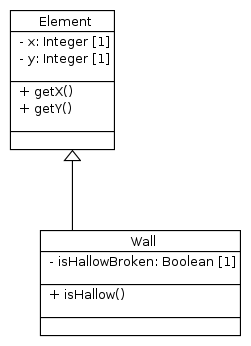
\includegraphics[scale=1]{./figure/model1.png} 


\begin{enumerate}
\item create(c1, Class)
\item addProperty(c1,name,'Element')
\item create(c2, Class)
\item addProperty(c2, name, 'Wall')
\item create(a1, Attribute)
\item addProperty(a1,name,'x');
\item addProperty(a1,type, 'Integer')
\item addProperty(a1, visibility, 'private')
\item addReference(c1, attribute, a1)

\item create(a2, Attribute)
\item addProperty(a2,name,'y');
\item addProperty(a2,type, 'Integer')
\item addProperty(a2, visibility, 'private')
\item addReference(c1, attribute, a2)

\item create(a3, Attribute)
\item addProperty(a2,name,'isHallowBroken');
\item addProperty(a2,type, 'Boolean')
\item addProperty(a2, visibility, 'private')
\item addReference(c2, attribute, a3)

\item create(m1, Method)
\item addProperty(m1,name,'getX');
\item addProperty(m1, visibility, 'public')
\item addReference(c1, attribute, m1)


\item create(m2, Method)
\item addProperty(m2,name,'getY');
\item addProperty(m2, visibility, 'public')
\item addReference(c1, attribute, m2)


\item create(m3, Method)
\item addProperty(m3,name,'isHallow');
\item addProperty(m3, visibility, 'public')
\item addReference(c2, attribute, m3)

\item addReference(c1,super,c2)
\end{enumerate}

2 étapes sont requises pour que 2 sites s'échangent des données. Premièrement, chaque site doit s'intégrer a un groupe. Cela leur permet de se voir et de communiquer. Deuxièmement, les 2 sites doivent utiliser D-Praxis pour voir les données locales de chacun. De ce fait, un site peut manifester un intérêt particulier pour un ou plusieurs éléments de ce modèle, ce qui revient à s'abonner à ces éléments. Ces éléments seront ensuite répliqués sur le site demandeur. Tous les changements effectués seront propagés aux sites abonnés. 
\newline
\newline
\newline
\newline Une fois encore, les modèles en D-Praxis sont représentés par une séquence d'opérations. Lorsqu' un site effectue un changement sur un  modèle au sein d'un groupe, les opérations correspondant à ces changements seront propagés aux abonnés partageant les mêmes éléments. Par souci d'optimisation, toutes les modifications ne sont pas propagées à tous les membres du groupe. Seuls les sites partageant les mêmes éléments qui ont été modifiés recevront ces modifications. L'intérêt de cette approche est qu'on diminue le nombre de messages échangés lors d'une modification. 
\subsubsection{Détection et Résolution de conflits}




\subsection{Telex}
Telex est un middleware développé au sein du de l'équipe Regal du LIP6. Telex est destiné aux applications de travail coopératif au sens large, c'est--dire qu'il n'est pas réservé  un type de document donné. Il permet à des utilisateurs répartis sur le réseau de partager des documents de manière optimiste. Le point fort de Telex, en plus de la gestion de la répartition et de la cohérence entre documents, c'est la possibilité de travailler en mode non-connecté. Cette fonctionnalité reflète au mieux la réalité des projets logiciels et répond  un vrai besoin des développeurs. Les développeurs peuvent travailler de leurs cotés puis se reconnecter et soumettre leur rendu  Telex et ce dernier se charge alors de trouver un consensus et converge vers un modèle compatible entre développeur.   
Pour construire une application sur Telex, il faut avant tout comprendre les notions basiques et l'architecture de Telex.
\subsubsection{Notions basiques}
Telex se base sur les concepts suivants : 
\begin{itemize}
\item Un \textbf{site} est une location où s'exécute une application Telex.
\item Une \textbf{action} est une opération réalisée sur une donnée partagée qui sera transmise  Telex.
\item Une \textbf{contrainte} est un invariant définissant les relations entre actions. 
\item Un \textbf{document} représente le "document" partagé entre sites. Dans sa structure interne, un document est un graphe orienté où les actions sont les nœuds du graphe et les contraintes représentesnt les arêtes.
\item Une \textbf{vue} est une représentation locale d'un document
\item Un \textbf{schedule} est une séquence d'actions générée par Telex qui seront exécutées par les applications. Lors d'un calcul d'un nouveau schedule, Telex calcule tous les 
chemins possibles entre les noeuds du graphe respectant les contraintes.
\end{itemize}
Telex, définit aussi 3 types de contraintes entre les actions : 
\begin{itemize}
\item \textbf{NotAfter} : A $\rightarrow$ B : A est n'est jamais après B dans n'importe quel schedule
\item \textbf{Enables} : A $\triangleleft$ B : Si B est dans un schedule implique A l'est aussi
\item \textbf{NonCommuting} : A $\nparallel$ B : ???
\end{itemize}
Ces contraintes peuvent être combinés pour obtenir :
\begin{itemize}
\item \textbf{Atomic} : A $\triangleleft$ $\triangleright$  B : Soit A et B s'exécutent sinon aucun des deux
\item \textbf{Causal} : A $\triangleleft$ $\rightarrow$  B : B s'exécute après A si et seulement si A réussit 
\item \textbf{Antagonisme} : A ( ?? ) B : Conflit : A et B ne seront jamais dans le même schedule
\end{itemize}

\subsubsection{Architecture}
Telex a été premièrement développé en Java en offrant une API mais cette dernière étant compliquée à utiliser qu'une autre version a été développée
appelé \textit{Telex Light Server} permettant aux applications de communiquer avec Telex grâce à des requêtes HTTP. L'avantage avec cette approche est 
que n'importe quelle application peut interagir avec Telex indépendamment de son langage d'implémentation. La réplication proprement dite est gérée entre les instances du serveur Telex partageant le même document.
\newline Le serveur Telex contient 4 composants :
\begin{itemize}
\item \textbf{Telex} : ce composant représente le cœur du serveur. Ce composant gère le document, calcule les nouveaux schedules, vérifie les contraintes entre actions et transmet 
ces actions aux autres instances du serveur partageant le même document. 
\item \textbf{ConstraintPooler} : ce composant contient une file de toutes les contraintes qui ont été soumises  à Telex.
\item \textbf{SchedulesPooler} : ce composant contient une file de de tous les schedules générés par Telex.
\item \textbf{MetaApp} : c'est un composant front-end entre le client et le serveur Telex. Ce dernier reçoit les requêtes HTTP du client  et se charge de les transmettre au composant Telex. 
\end{itemize}

Il existe un autre composant qu'on peut intégrer coté client mais qui n'est pas nécessaire dans le fonctionnement de Telex. Ce composant est appelé le \textbf{reflector} et c'est lui qui assure l'aspect déconnecté de Telex. Ce composant s'utilise de manière transparente coté client. Un client peut décider à tout moment de se déconnecter de Telex et travailler sur son espace en local. Le client crée des actions, des contraintes, génère de nouveaux schedules et les soumet au reflector de manière transparente. Lors de la reconnection, le reflector soumet à Telex les nouvelles actions et contraintes à Telex et reçoit les nouvelles actions et contraintes des autres instances de Telex. C'est à ce stade que des conflits peuvent être identifiés que Telex proposera ensuite des solutions à leurs résolutions.
L'architecture finale de Telex est décrite ici : 

<!-- include images architecture Telex -->


\subsubsection{Telex : Commandes}
Une application voulant utiliser Telex doit respecter le protocole Telex. Ce protocole est basé sur l'XML et accepte les opérations suivantes :
\begin{itemize}
\item \textbf{INIT} : permet d'initialiser le dialogue avec le serveur.
\item \textbf{OPEN} : permet d'ouvrir un document sur Telex. Cette commande prend 2 paramètres obligatoires : le nom du document et son mode d'ouverture, \textit{R} pour ouvrir en lecture et \textit{R/W} pour ouvrir en lecture-écriture.
\item \textbf{ACTION} : permet de soumettre des actions  Telex. Cette commande prend 2 paramètres obligatoires qui sont le nom de l'action  et son identifiant. L'identifiant de l'action est un entier.
\item \textbf{AFRAG} : permet de soumettre un fragment à Telex. On soumet un fragment avec une ou plusieurs actions ainsi que les contraintes entre ces actions. Elle assure que les actions et les
contraintes soumises seront écrites dans le document et se fera de manière atomique.
\item \textbf{GETLASTSCHEDULES} : retourne la liste des schedules générés par Telex. Elle ne prend pas de paramètre. 
\item \textbf{CONSTR} : permet de soumettre des contraintes entre actions. Elle prend le nom de la contrainte, le type de la contrainte (NOT-AFTER, ENABLES, NON-COMMUTING) et les actions concernées.
\item \textbf{GETCONSTR} : renvoie la liste des actions ayant le même identifiant. 
\end{itemize}

La commande ACTION ne suffit pas pour que Telex reconnaisse l'action, c'est à dire présent dans le graphe de document. Il est obligatoire de le soumettre avec la commande AFRAG pour assurer qu'elle sera présente.  
Quelques exemples de commandes Telex :

\begin{lstlisting}[caption=Un exemple de commande pour ouvrir un document sur Telex]
<commands>
<command>
		<name>OPEN</name>
		<param> myDocument</param>
		<param>R/W</param>
	</command>
</commands>
\end{lstlisting}


\begin{lstlisting}[caption=Un autre exemple de commande permettant de soumettre plusieurs actions à Telex dans un fragment]
<?xml version="1.0" encoding="UTF-8"?>
<commands>
	<command>
		<name>ACTION</name>
		<param>CREATE_CLASS_A</param>
		<param><1</param>
	</command>
	<command>
		<name>ACTION</name>
		<param>CREATE_CLASS_B</param>
		<param><2</param>
	</command>
	<command>
		<name>ACTION</name>
		<param>ADDPROPERTY_B_TO_CLASS_A</param>
		<param><1</param>
	</command>
	<command>
		<name>ACTION</name>
		<param>ADDPROPERTY_B_TO_CLASS_A</param>
		<param><1</param>
	</command>
	<command>
		<name>AFRAG</name>
		<param>myDocument</param>
		<param>CREATE_CLASS_A</param>
		<param>CREATE_CLASS_B</param>
		<param>ADDPROPERTY_B_TO_CLASS_A</param>
	</command>
</commands>
\end{lstlisting}

\subsubsection{Telex : Workflow}
Nous allons montrer à travers un exemple comment fonctionne Telex. On va pour cela supposer que 2 clients interagissent avec 2 instances de Telex : C1 avec le serveur S1 et C2 avec le serveur S2. Ces 2 serveurs se partageront un document appelé Doc.
\newline C1 commence par se connecter au serveur S1 en envoyant la commande INIT et pour ouvrir le document avec la commande OPEN.C1 soumet ses actions A_1 avec la clé 1 et B\_2 avec la clé 2. Ces actions seront ajoutées dans un fragment et transmises à la MetaApp. On rappelle que le fragment sert à garantir l'unicité d'écriture dans le document. La MetaApp réçoit ces actions et les transmet à Telex. Telex les récupère, les écrit dans le document Doc. Telex calcule ensuite un nouveau schedule et le transmet à la MetaApp. Le nouveau schedule calculé sera inséré dans le SchedulesPooler. Un appel avec la commande GETLASTSCHEDULE renverra la combinaison A_1 et B_1 ou B_1 et A_1 étant donné il n'existe aucune contrainte entre A_1 et B_1. Voici comment est représenté le graphe du document Doc :

<!-- images graphe document-->
Le client C2 se connecte à S2 et ouvre le document Doc par le meme procédé que S1. Automatiquement, les actions se trouvant S1 sont propagés sur S2. Telex coté S2 se charge d'écrire ses actions sur le Doc et de générer un nouveau schedule qui sera le meme coté S1. 

<!--- image -->

C2 soumet une action X_1 avec la clé 1. La MetaApp transmet les actions à Telex qui se charge de les écrire dans le document, calcule un nouveau schedule et envoie cette action à S1. Lors de l'appel de GETLASTSCHEDULE, la réponse envoyée sera une combinaison des 3 : X_1, A_1, B_1. Etant donné que les actions X_1 et A_1 ont les memes clés, elles seront insérées dans le ConstraintPooler, des 2 cotés. Un appel à la commande GETCONSTRAINT  renverra X_1 et A_1. 
<!-- une autre image -->

 C2 souhaite mettre une contrainte NOT-AFTER entre X_1 et A_1 tel que X_1 $\rightarrow$ A_1. La contrainte NOT-AFTER signifie que l'action A_1 ne peut se réaliser ou apparaitre dans un schedule avant X_1. Telex écrit cette contrainte dans le document, le transmet à S1 et génère un nouveau schedule. Le nouveau schedule généré sera : X_1,A_1,B_2, ou encore X_1,B_2,A_1. Notre graphe de documents se dessine comme suit :
 
 <!-- images -->
 
 C1 décide de soumettre la contrainte NON-COMMUTING entre A_1 et B_2 tel que A_1 et B_2. La contrainte NON-COMMUTING ????. Donc encore une fois, Telex reçoit cette contrainte, l'écrit dans le document, le transmet à S2 et génère un nouveau schedule. Le nouveau schedule sera soit .....
 
 <!-- images -->
 
 Voici comment fonctionne Telex. Donc, un client utilisant Telex doit à chaque fois faire appel aux commandes GETCONSTR et GETLASTSCHEDULES pour connaitre quelles sont les actions à exécuter. C'est ce que nous avons fait en portant D-Praxis sur Telex.
 
  
\section{GraphElex : D-Praxis over Telex}
\subsection{Réplication totale}
\subsection{Réplication partielles}





% Bibliographie
%\bibliographystyle{alpha}
%\bibliography{biblio}



\end{document}











